\label{flushing_case_study}
When a water utility becomes aware of a water quality issue either through 
customer complaints or water quality sensor alarms, they often open a hydrant to 
flush a portion of the distribution network in order to bring new water into the 
area and increase the chlorine residual. This case study examines how WST can 
be used to identify effective flushing locations following a water quality 
sensor alarm using the the \code{flushing}, \code{inversion} and 
\code{grabsample} subcommands. All files required to run the case study 
are provided in the \code{examples/case\_studies/flushing} folder.

The EPANET input file for this example is Net6.inp, which has a simulation duration 
of seven (7) days starting at midnight. The network is assumed to include a contamination 
warning system (CWS) with ten optimally placed water quality sensors and an 
event detection system in operation. The 10 sensors are located at 
JUNCTION-1617, JUNCTION-199, JUNCTION-2297, 
JUNCTION-2716, JUNCTION-2930, JUNCTION-3023, JUNCTION-435, JUNCTION-552, 
JUNCTION-675 and JUNCTION-831. The sensors were optimally placed 
using the \code{sp} subcommand. 
Figure \ref{fig:wds_sensors} shows the water distribution network and the location of the 
water quality sensors. The CWS provides binary values every 15 minutes from each sensor 
location. The binary value is zero if water quality conditions 
are normal or one if the conditions are abnormal.  

\begin{figure}[h!]
\begin{center}
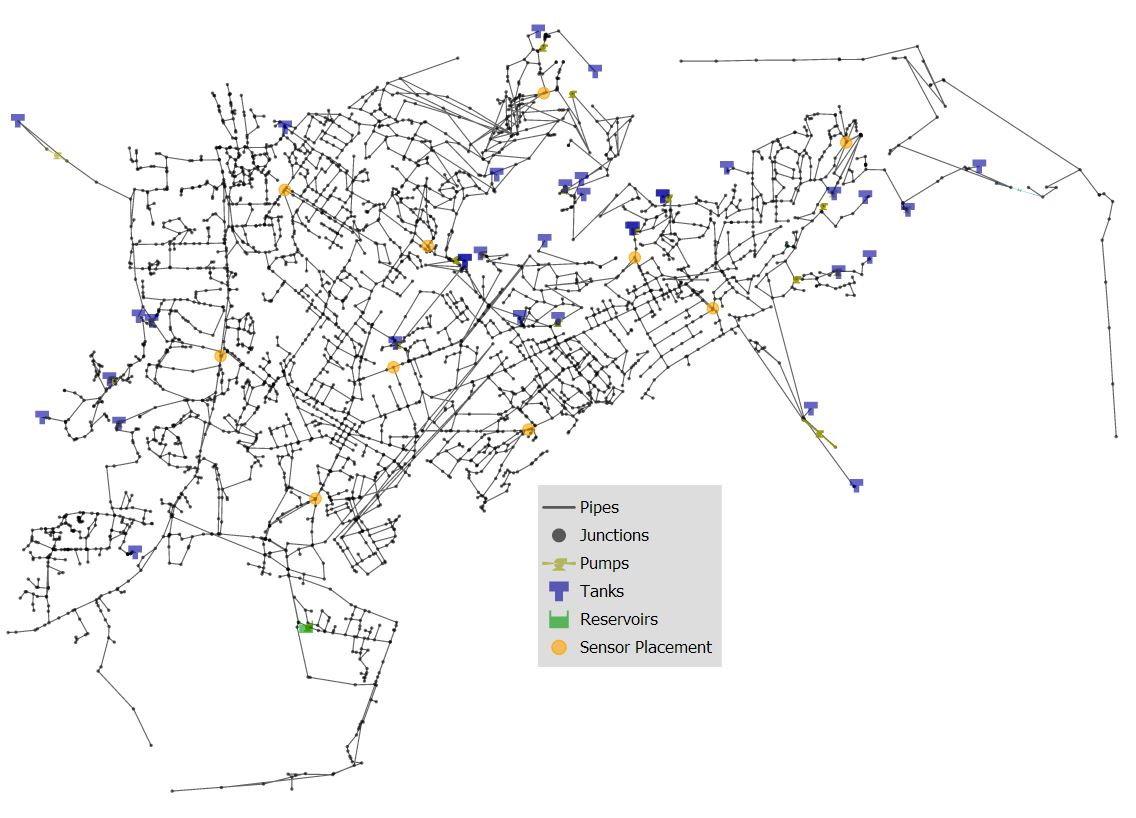
\includegraphics[scale=0.6]{graphics/Net6_Sensors.JPG}
\caption{Net6 water distribution network with water quality sensors.}
\label{fig:wds_sensors}
\end{center}
\end{figure}
 
At 10:15 AM, the CWS alerts water utility staff to abnormal water quality occurring 
at water quality sensor located at JUNCTION-1617 in water distribution network model. 
Figure \ref{fig:wds_sensors_detect} shows the JUNCTION-1617 highlighted as the sensor 
location with a positive detection of contamination in the network.  

\begin{figure}[h!]
\begin{center}
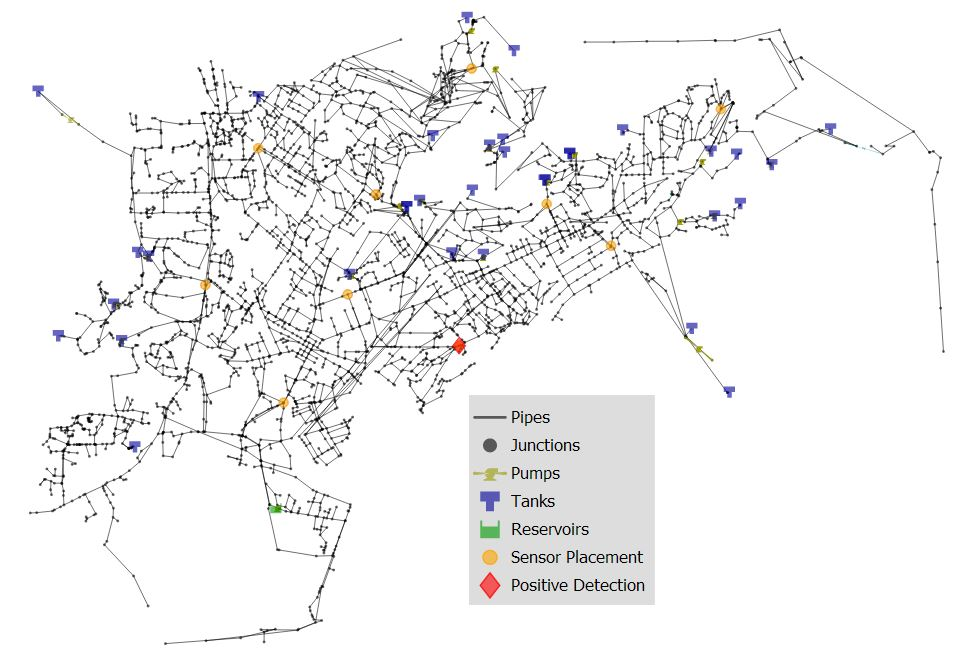
\includegraphics[scale=0.6]{graphics/Net6_Sensors_detect.JPG}
\caption{Net6 with positive contamination detection at JUNCTION-1617.}
\label{fig:wds_sensors_detect}
\end{center}
\end{figure}

The water utility must now decide how to proceed. The staff checks their 
consequence management plan and sends out a team to ensure that the water quality 
sensor is working properly. The water utility staff determines 
that a contamination incident is possible and they would like to identify the source.  
Source identification allows the water utility to determine the extent of contamination (or spread) and possibly
shut off any continuing injection of contaminants.  
Using the CWS information from the past 35 hours, provided in the measurements file 
Net6\_CWS\_MEASURES.dat, and the Net6 INP file, the \code{inversion} subcommand is used to 
identify the possible sources of the contamination. The inversion configuration file, 
Net6\_inversion.yml, and the measurements file are provided in the \code{examples/case\_studies/flushing} folder.

The \code{inversion} subcommand can be executed using the following command line:

\begin{unknownListing}
wst inversion Net6_inversion.yml
\end{unknownListing}  

Figure \ref{fig:wds_sources} shows the 25 possible contamination sources identified by the 
\code{inversion} subcommand.  

\begin{figure}[h!]
\begin{center}
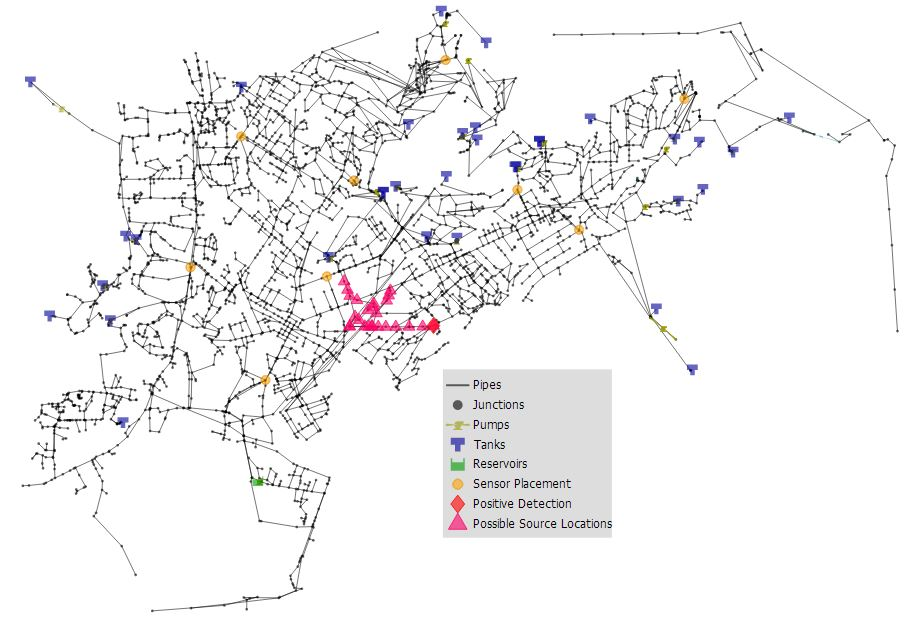
\includegraphics[scale=0.6]{graphics/Net6_possible_sources.JPG}
\caption{Net6 with possible contamination sources identified by \code{inversion} subcommand.}
\label{fig:wds_sources}
\end{center}
\end{figure}

Since flushing is a common response to abnormal water quality, the water utility staff decide 
to open hydrants to flush the contaminated water out of the network. To determine the most 
effective flushing locations, the staff simulates contamination incidents from each 
possible contamination source location using the TSG file produced from the \code{inversion} subcommand. 
From these simulations, the possible extent of contamination from each source location is identified. 
The nodes in the water distribution network model which are calculated to have 
contaminant concentrations above zero at the starting of flushing (12:00 PM, 
approximately two hours after detection) are considered as the initial starting points for the network 
solver option in the \code{flushing} subcommand. These initial starting points 
are the first node locations that are going to be evaluated in terms of the impact metric  
and then as the process continues, the solver will look at all of the nodes that are 
connected to these initial points to determine their impact metrics. Figure \ref{fig:wds_impacted_nodes} 
shows the nodes impacted by the 25 possible contamination source locations.  

\begin{figure}[h!]
\begin{center}
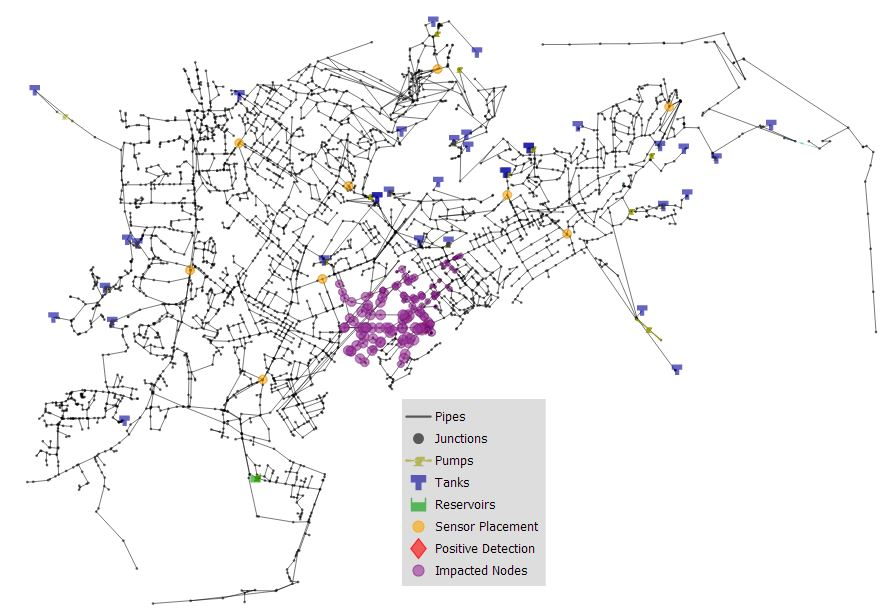
\includegraphics[scale=0.6]{graphics/Net6_imapcted_nodes_25inj.JPG}
\caption{Net6 with nodes impacted by the 25 possible contamination sources.}
\label{fig:wds_impacted_nodes}
\end{center}
\end{figure}

The water utility decides to open two hydrants to flush the contaminated water out of the network, 
since the extent of contamination for the possible 25 contamination sources (as seen in 
Figure \ref{fig:wds_impacted_nodes}) is not very large at the 
start of flushing at 12:00 PM. To identify effective 
flushing locations, the \code{flushing} subcommand is used. This command requires the following 
files as specified in the flushing configuration file, Net6\_flush\_2nodes.yml:

\begin{itemize}
\item Net6.inp - Net6 EPANET input (INP) file.
\item Net6\_inv1\_profile.tsg - The TSG file created by the \code{inversion} subcommand.
\item Net6\_bio.tai - The TAI file describing the dose-response characteristics for the assumed contaminant. 
This file is required when using the population exposed (PE) impact metric. 
\end{itemize}  

In addition, characteristics of the flushing response are also defined in the 
flushing configuration file. These include:

\begin{itemize}
\item A list of nodes that can be flushed - All non-zero demand (NZD) nodes 
\item The maximum number of nodes which can be flushed simultaneously - 2 
\item The flushing rate - 1100 gallons/min
\item The flushing duration - 8 hours 
\item The response time delay (time between detection and start of flushing) - 1 hour
\end{itemize}  

Other information provided in the flushing configuration file include the 
impact metric that is going to be minimized (PE), the nodes where water 
quality sensors are located, the type of solver (network solver), 
and the initial starting points for the network solver (JUNCTION-1881 and 
JUNCTION-1878). 

The \code{flushing} subcommand can be executed using the following command line:

\begin{unknownListing}
wst flushing Net6_flush_2nodes.yml
\end{unknownListing}  

Figure \ref{fig:wds_flushing_nodes} shows the flushing nodes identified by 
the \code{flushing} subcommand. The flushing nodes identified are JUNCTION-1881 
and JUNCTION-2233.  

\begin{figure}[h!]
\begin{center}
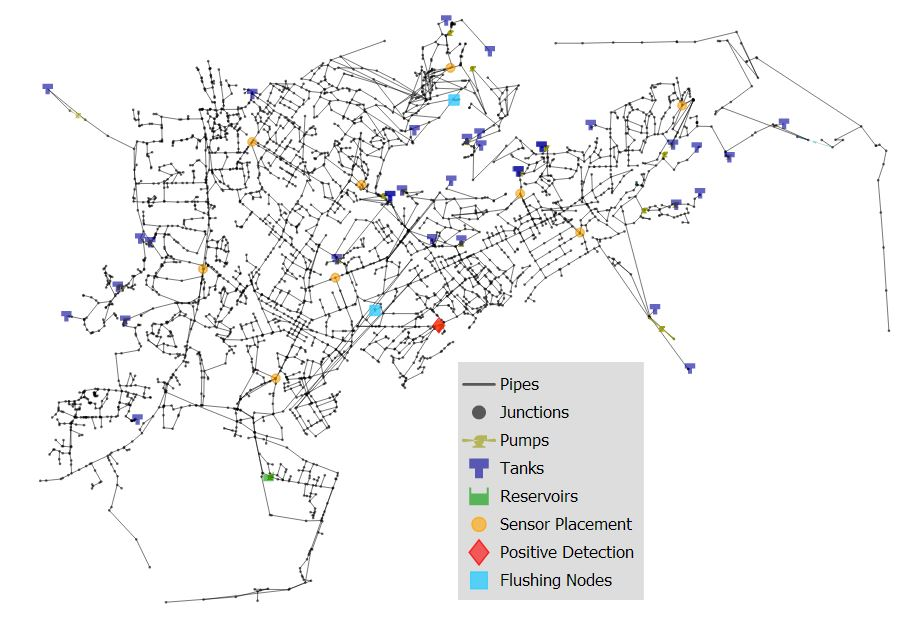
\includegraphics[scale=0.6]{graphics/Net6_2nodes_flushing.JPG}
\caption{Net6 with the flushing nodes identified by the \code{flushing} subcommand.}
\label{fig:wds_flushing_nodes}
\end{center}
\end{figure}

Since the identified flushing nodes were based upon the 25 possible contamination sources, 
the water utility staff evaluate the flushing response against each of the possible 
sources assuming it was the true source of the contamination. This option is available 
using EVALUATE as the type under the solver block of the flushing configuration file. An 
example flushing configuration file for the evaluate option is provided in 
Net6\_flush\_2nodes\_eval\_JUNC1617.yml in the \code{examples/case\_studies/flushing} folder. 
This example assumes that JUNCTION-1617 is the true source of contamination in the network 
and it evaluates the effectiveness of the identified flushing locations in terms of the 
PE metric. If JUNCTION-1617 is the true source, flushing at JUNCTION-1881 and JUNCTION-2233 
reduces the PE metric by only two percent (2\%).

% \todo{can you assume a different true source?  This one is among the worst.}

The \code{flushing} subcommand for this example can be executed using the following command line:

\begin{unknownListing}
wst flushing Net6_flush_2nodes_eval_JUNC1617.yml
\end{unknownListing}

Because the \code{inversion} subcommand solvers assume a continuous injection, the 
created TSG file has the contamination injection durations lasting as long as the 
simulation duration listed in the network INP file. Thus, the contamination injections 
start a little before the detection time and stop at the end of the simulation 
(seven days). Since an important response action would include shutting off the 
source of contamination, the TSG file is modified to stop the injection five 
hours after detection. Using the modified TSG file, the flushing response is evaluated 
against each of the 25 possible sources assuming it was the true source of the contamination.   
Figure \ref{fig:flushing_pe_reduction} shows the percent reduction in the PE metric 
for each of the 25 possible contamination sources with flushing alone (blue) and 
flushing with shutting off the contamination source (green). The percent 
reduction in the PE metric ranges from 24\% to 97\% for the flushing with source shut-off 
response action, which is an increase from the range of 2\% to 45\% for the flushing alone 
action. The highest percent reduction was if the true injection incident occurred at JUNCTION-1881.

\begin{figure}[h!]
\begin{center}
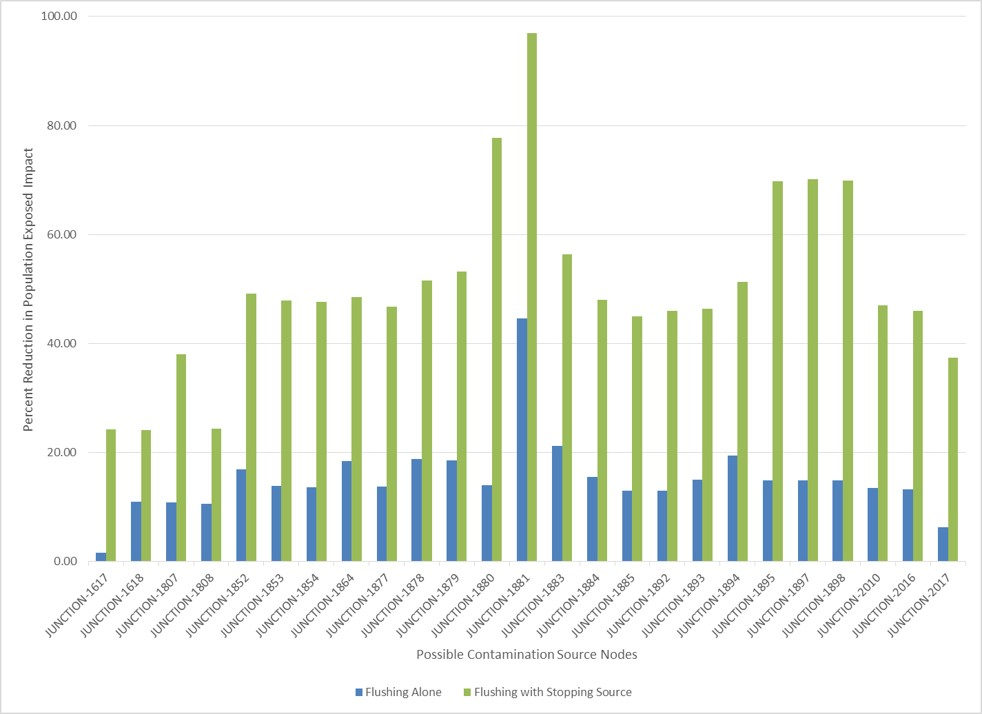
\includegraphics[scale=0.6]{graphics/flushing_pe_reduction.jpg}
\caption{The reduction in the PE metric for each of the 25 possible contamination sources.}
\label{fig:flushing_pe_reduction}
\end{center}
\end{figure}

% If the water utility wants to reduce the number of possible contamination sources 
% and improve the effectiveness of the flushing response, they could send staff to 
% manually collect grab samples to supplement the CWS measurements. 
 
% \todo{was grabsample used?}
